\chapter{Finite Element Method For Rotordynamic systems}
In this chapter the Finite Element Method(FEM) will be employed in the simulation of rotordynamic systems. There are many advantages to using this discretizing method to solve problems of rotating machines. One of which is the generic form that the equation, and its parts take. The method lends itself to being able to easily create new matrices that can insert right into your equations of motion. Another, is the ability to move components around in space without the need to reevaluate the physics. Finally, the analysis techniques for Multiple Degree Of Freedom (MDOF) systems is wide reaching, and will serve to richly enhance our understanding of a complex system made of simple parts.\par 
First, the beam element commonly refered to as the Timoshenko Beam Element will be derived from the kinematic and constitutive constraints (An alternative element, the Bernoulli-Euler element is provided in Appendix A). Then the solution to the resulting equation of motion will be discretized and variables separated in position and time to give the finite element equations of motion. Further, an extension to the beam element model is presented that will consider the viscous damping effects in the beam element. Equations for disks, bearings, and complex versions of all equations will be presented. Finally, the assembly and analysis of the model will result in intuitive figures that will be shown to compare well to experimental data.
\section{Timoshenko Beam Finite Element} \label{Timoshenko Beam Finite Element}
The Timoshenko beam element allows for the beam cross section plane at any axis location to differ from normal with the axis of the beam. In other words, the element allows for shear stresses. This element often also includes the effects of rotary inertia and gyroscopic moments, as it will in this derivation. Generalized displacements used are assumed to be variable in both time and space. The element has six degrees of freedom. Three translation and three rotations all defined on the beam axis. So then all displacements are functions of time, $ t $, and the axial spacial coordinate, $ x $.
\subsection{Kinematic Relationships} \label{Kinematic Relationships}
\begin{figure}
	\centering
	\def\svgwidth{400pt}
	\import{figures/}{kinematicbeamsurface.pdf_tex}
	\caption{Beam Element with nodal displacements.}
	\label{fig:KineBeamElem}
\end{figure}
\begin{figure}
	\centering
	\def\svgwidth{250pt}
	\import{figures/}{TimoBeamDOF.pdf_tex}
	\caption{Timoshenko beam section with degrees of freedom at some point x along beam axis.}
	\label{fig:TimoBeamDOF}
\end{figure}
In order to develop the stresses and strains internal to the beam, and subsequently the equations of motion, the motion of some arbitrary point on the beam must be defined in terms of the generalized coordinates. Motion of two points is taken into consideration to assist in dividing the motion into a translation and a rotation. These points are shown in Figure \ref{fig:KineBeamElem}. The first point, $ C $, falls on the beam axis at location x, and in the undeformed configuration, the vector $ \vec{r}_c^\prime= \overrightarrow{OC} $ forms a right angle with the surface of the cross section. The second point, $ P $ is at some arbitrary $ (y,z) $ location on the cross section. The vecor $ \vec{t}=\overrightarrow{CP} $ points from the beam axis to the point along the cross section. If we follow this point $ P $ we will be able to define the motion of the cross section as a whole, or more succinctly, to define the displacements $ u_p,v_p,w_p $ in terms of the coordinates $ u,v,w,\psi,\theta$, \& $\phi $. The motion of point P is split into translation and rotation, where $ \vec{t} $ is rotated and $ \vec{r}_c $ is translated to point to the deformed location $ P' $. The vector pointing to P in the undeformed state is defined as
\begin{equation}\label{eq:r}
\vec{r}=\vec{r}_c+\vec{t}
\end{equation}
Rotations are represented with a rotation transformation matrix,
\begin{equation}\label{eq:trot}
\vec{t}^\prime=\underline{R}\vec{t}
\end{equation}
The linearized first order rotational matrix for small angles is represented by 
\begin{equation}\label{eq:RotTransformation}
\underline{R}=\left[\begin{array}{ccc}
1&-\theta&\psi\\
\theta&1&-\phi\\
-\psi&\phi&1
\end{array}\right]
\end{equation}
and the translation with a displacement vector 
\begin{equation}\label{eq:rtrans}
\vec{r}_c^\prime=\vec{r}_c+\vec{u}
\end{equation}
%\begin{equation}\label{eq:RotTransformationExpanded}
%R=\underline{I}+\tilde{\underline{\Psi}}+1/2\left(\tilde{\underline{\Psi}}\right)^2+...
%\end{equation}
%\begin{equation}\label{eq:RotTransformationApprox}
%R\approx\underline{I}+\tilde{\underline{\Psi}}
%\end{equation}
Combined motion from $ P $ to $ P' $ can be defined by
\begin{equation}\label{eq:DispVectorrpr}
\vec{u}_p=\vec{r^\prime}-\vec{r}
\end{equation}
where $ \vec{u}_p  $ is the vector containing $ u_p,\:v_p,\:\&\:w_p $. The vector definitions for $ \vec{r}' $ and $ \vec{r} $ are substituted to the above equation to obtain
\begin{equation}\label{eq:DispVectorrptprt}
\vec{u}_p=\vec{r_c^\prime}+\vec{t^\prime}-\vec{r}_c+\vec{t}
\end{equation}
and now using the definition for $ \vec{u} $ and $ \vec{t}' $ leads to the simplified expression for the motion of $ P $
\begin{equation}\label{eq:DispVectRotTranst}
\vec{u}_p=\vec{u}+(\underline{R}-\underline{I})\vec{t}
\end{equation}
expanding matrices reveals the equation
\begin{equation}\label{DispVectExpanded}
\vec{u}_p = \left\{\begin{array}{c}
	u_p\\
	v_p\\
	w_p\end{array}\right\}=\left\{\begin{array}{c}
	u\\
	v\\
	w\end{array}\right\}+\left[\begin{array}{ccc}
	0&-\theta&\psi\\
	\theta&0&-\phi\\
	-\psi&\phi&0
	\end{array}\right]\left\{\begin{array}{c}
	0\\
	y\\
	z\end{array}\right\}
\end{equation}
Therefore, the motion of any point on the beam may be approximated with
\begin{equation}\label{eq:DispVectEvaluated}
\vec{u}_p=\left\{\begin{array}{c}
u-\theta y+\psi z\\
v-\phi z\\
w+\phi y\end{array}\right\}
\end{equation}
\subsection{Internal Constitutive Relationship} \label{Internal Constitutive Relationship}
Stresses are assumed to exist in the beam in the axial direction, and in shear on the face of the beam section. Stresses in the transverse, or the y and z, directions are assumed negligible. Shear stresses out of the plane section are assumed to be vanishing as the differential element shrinks. Internal damping is to be considered independently from this material constitutive relationship. Written out, these stresses are represented by the matrix
\begin{equation}\label{key}
\sigma_{ij}=\left[\begin{array}{ccc}
\sigma_{xx}&\sigma_{xy}&\sigma_{xz}\\
\sigma_{xy}&0&0\\
\sigma_{xz}&0&0
\end{array}\right]
\end{equation}
using the Hooke's Law for a linear elastic isotropic material, expressed as
\begin{equation}\label{key}
\epsilon_{ij}=\frac{1}{E}[(1+\nu)\sigma_{ij}-\nu\delta_{ij}\sigma_{kk}]
\end{equation}
allows the determination of the stress strain relationship in engineering notation as
\begin{equation}\label{eq:ConstitutiveRelationshipEngineeringNotation}
\left\{\begin{array}{c}
\sigma_{xx}\\ \sigma_{xy}\\ \sigma_{xz}
\end{array}\right\} = \left[\begin{array}{ccc}
E&0&0\\0&2G&0\\0&0&2G
\end{array}\right] \left\{\begin{array}{c}
\epsilon_{xx}\\ \epsilon_{xy}\\ \epsilon_{xz}
\end{array}\right\}
\end{equation}
where, $ G=\frac{E}{2(1+\nu)} $. Strains are derived from displacements of equation \eqref{eq:DispVectEvaluated} using a linear strain-displacement relationship for infinitesimal strains: $ 2\epsilon_{ij}=u_{i,j}+u_{j,i} $.
%\begin{equation}\label{eq:LinearStrainDispRelationship}
%
%\end{equation}
%\begin{equation}\label{eq:StrainEvaluated}
%\underline{\epsilon}=\frac{1}{2}\left[\begin{array}{ccc}
%2\left(\frac{\partial u_c}{\partial x}-\frac{\partial\theta}{\partial x}y+\frac{\partial\psi}{\partial x}z\right) & \frac{\partial v_c}{\partial x}-\frac{\partial\phi}{\partial x}z-\theta & \frac{\partial w_c}{\partial x}+\frac{\partial \phi}{\partial x}y+\psi\\
%\frac{\partial v_c}{\partial x}-\frac{\partial\phi}{\partial x}z-\theta &0&0\\
%\frac{\partial w_c}{\partial x}+\frac{\partial \phi}{\partial x}y+\psi&0&0\end{array}\right]
%\end{equation}
\begin{equation}\label{eq:StrainEvaluatedSimple}
\left\{\arraycolsep=1pt\begin{array}{rl}
\epsilon_{xx}&=u'-\theta'y+\psi'z\\
\epsilon_{xy}&=\frac{1}{2}(v'-\phi'z-\theta)\\
\epsilon_{xz}&=\frac{1}{2}(w'+\phi'y+\psi)
\end{array}\right.
\end{equation}
Note that in the case of the Euler-Bernoulli beam derivation the slope in a transverse direction displacement is equal to the rotation angle about the orthogonal transverse axis, i.e., $v'=\theta$ and $w'=\psi$. Application of those would reduce the system to the Euler-Bernoulli beam.\par

It will be proven useful to introduce generalized strains that group strain contributions above as axial, bending, torsion, and shear, represented by the symbols $ \varepsilon $, $ \rho $, $ \varphi $, $ \gamma $,respectively.
\begin{equation}\label{eq:GeneralizedStrains}
\left\{\arraycolsep=1pt\begin{array}{rl}
\varepsilon&=u'\\
\rho_{y}&=-\theta'\\
\rho_{z}&=\psi'\\
\varphi&=\phi'\\
\gamma_{y}&=v'-\theta\\
\gamma_{z}&=w'+\psi\end{array}\right.
\end{equation}
allowing the representation of the strains from eq \eqref{eq:StrainEvaluatedSimple} using the generalized strains as:
\begin{equation}\label{eq:StrainEvaluatedSimpleGeneralized}
\left\{\begin{array}{l}
\epsilon_{xx}=\varepsilon+\rho_yy+\rho_zz\\
\epsilon_{xy}=\frac{1}{2}(\gamma_y-\varphi z)\\
\epsilon_{xz}=\frac{1}{2}(\gamma_z+\varphi y)
\end{array}\right.
\end{equation}
Now the stresses in equation \eqref{eq:ConstitutiveRelationshipEngineeringNotation} can be represented with the displacements as 
\begin{equation}\label{key}
\left\{\begin{array}{c}
\sigma_{xx}\\ \sigma_{xy}\\ \sigma_{xz}
\end{array}\right\} = \left\{\begin{array}{c}
E(u'-\theta'y+\psi'z)\\ G(v'-\phi'z-\theta)\\ G(w'+\phi'y+\psi)
\end{array}\right\} = \left\{\begin{array}{c}
E(\varepsilon+\rho_yy+\rho_zz)\\ G(\gamma_y-\varphi z)\\ G(\gamma_z+\varphi y)
\end{array}\right\}
\end{equation}
%Stress at the beam axis is expressed using Hooke's Law for linear isotropic homogeneous material
%\begin{equation}\label{LinearElasticStressStrainRelationship}
%\sigma_{ij}=\lambda\delta_{ij}\epsilon_{kk}+2\mu\epsilon_{ij}
%\end{equation}
%expanded out 
%\begin{equation}\label{StressEvaluated}
%\underline{\sigma}=\left[\begin{array}{ccc}
%(\lambda+2\mu)(u'-\theta'y+\psi'z)&\mu(v'-\phi'z-\theta)&\mu(w'+\phi'y+\psi)\\
%\mu(v'-\phi'z-\theta)&\lambda(u'-\theta'y+\psi'z)&0\\
%\mu(w'+\phi'y+\psi)&0&\lambda(u'-\theta'y+\psi'z)
%\end{array}\right]
%\end{equation}
%\begin{equation}\label{key}
%\sigma_{ij}=\lambda\delta_{ij}\epsilon_{k,k}+\mu\left(u_{i,j}+u_{j,i}\right)
%\end{equation}
\begin{equation}\label{eq:TotalVirtualStrainEnergyExpression}
U = \int_{\volume}\sigma_{ij}\epsilon_{ij}d\volume
\end{equation}
Now the inner product of the total virtual strain energy can be expanded
\begin{equation}\label{eq:TotalStrainEnergyExpanded}
U=\int_{\volume}\left[\sigma_{xx}\epsilon_{xx}+2\sigma_{xy}\epsilon_{xy}+2\sigma_{xz}\epsilon_{xz}\right]d\volume
\end{equation}
Then expand virtual strains into the generalized strains corresponding to the degrees of freedom of the beam element and collect terms on generalized strains
\begin{equation}\label{eq:TotalStrainEnergyGeneralized}
 U=\int_{\volume}\left[\sigma_{xx}\varepsilon+\sigma_{xx}y\rho_y+\sigma_{xx}z\rho_z+\sigma_{xy}\gamma_y+\sigma_{xz}\gamma_z+(\sigma_{xz}y-\sigma_{xy}z)\varphi\right]d\volume
\end{equation}
this internal mechanical energy expression allows us to recognize stresses conjugate with each generalized strain as the corresponding stress for that phenomena. Integration allows the determination of the forces and moments related to each generalized strain as
\begin{equation}\label{eq:generalizedForces}
\left\{\arraycolsep=1pt\begin{array}{rcl}
N=&\int_A\sigma_{xx}dA&=E( A\varepsilon+S_y\rho_y+S_z\rho_z)\\
M_y=&\int_A\sigma_{xx}zdA&=E(S_z\varepsilon+I_{xy}\rho_y+I_y\rho_z)\\
M_z=&\int_A\sigma_{xx}ydA&=E(S_y\varepsilon+I_z\rho_y+I_{xy}\rho_z)\\
Q_y=&\int_A\sigma_{xy}dA&=\kappa G(A\gamma_y-S_z\varphi)\\
Q_z=&\int_A\sigma_{xz}dA&=\kappa G(A\gamma_z+S_y\varphi)\\
M_x=&\int_A(\sigma_{xz}y-\sigma_{xy}z)dA&=\kappa G\left(A_y\gamma_z-A_z\gamma_y+J_x\varphi\right)
\end{array}\right.
\end{equation}
\begin{center}where, $ \left\{\begin{array}{l}
\ \kappa=\frac{6(1+\nu)}{7+6\nu}, \textit{for circular cross sections.}\\
\arraycolsep=.75pt\begin{array}{rlccccrl}
A&=\int_AdA&&&&&S_y&=\int_A ydA\\
S_z&=\int_AzdA&&&&&I_y&=\int_Az^2dA\\
I_z&=\int_Ay^2dA&&&&&J_x&=I_y+I_z
\end{array}
\end{array}\right. $\\\end{center}
$ \kappa $ is the shear coefficient which attempts to correct for the fact that the shear strain is not constant over the beam cross section. Assuming the central axis of the beam is coincident with the shear center, then $ A_y=A_z=I_{xy}=0 $. Which simplifies the conjugate forces to


\begin{equation}\label{eq:generalizedForcesSimplified}
\left\{\arraycolsep=1pt\begin{array}{rll}
N&=EA\varepsilon&=EAu'\\
M_y&=EI_y\rho_z&=EI_y\psi'\\
M_z&=EI_z\rho_y&=-EI_z\theta'\\
Q_y&=\kappa G A\gamma_y&=\kappa G A(v'-\theta)\\
Q_z&=\kappa G A\gamma_z&=\kappa G A(w'+\psi)\\
M_x&=\kappa G J_x\varphi&=\kappa G J_x\phi'
\end{array}\right.
\end{equation}

%\begin{equation}\label{eq:TotalVirtualStrainEnergyGeneralizedExpanded}
%\delta U=\int_{0}^{l}\left[N\delta\varepsilon+M_z\delta\rho_y+M_y\delta\rho_z+Q_y\delta\gamma_y+Q_z\delta\gamma_z+M_x\delta\varphi\right]dx
%\end{equation}
%upon expanding with forces defined in eq \eqref{eq:generalizedForcesSimplified}
%\begin{multline}
%\delta U=\int_{0}^{l}[EAu'\delta u'
%+EI_y\psi'\delta\psi'
%+EI_z\theta'\delta\theta'
%+\kappa G A(v'-\theta)(\delta v'-\delta\theta)\\
%+\kappa G A(w'+\psi)(\delta w'+\delta\psi)
%+\kappa G J_x\phi'\delta\phi']dx
%\end{multline}
%and using integration by parts to achieve a relation to the displacements 
%\begin{multline}\label{eq:TotalVirtualStrainEnergyDisplacementRel}
%\delta U=\int_{0}^{l}\{EAu''\delta u
%+\kappa G A(v''-\theta')\delta v
%+\kappa G A(w''+\psi')\delta w\\
%+[EI_y\psi''-\kappa G A(w'+\psi)]\delta\psi
%+[EI_z\theta''+\kappa G A(v'-\theta)]\delta\theta\\
%+\kappa G J_x\phi''\delta\phi\}dx + \delta U_b
%\end{multline}
%leaving $ \delta U_b $ as the boundary value terms to be neglected. The principle of virtual work for a quasistatic beam with no external work gives $ \delta U=0 $. Therefore, each term in the integrand of \eqref{eq:TotalVirtualStrainEnergyDisplacementRel} must equal zero.
\subsection{Differential Equations of Motion} \label{Differential Equations of Motion}
Now the equations are motion are derived for the Timoshenko beam element. External forces are not included in this derivation. Though they may easily be added to the diagram of figure \ref{fig:BeamDifferentialSection} and included in the analysis. It is also assumed that the cross section remains planar during deformation and the material properties are homogeneous through time and space. The derivation is the same as for a Euler-Bernoulli beam with the exception of the constitutive relations used at the end and the inclusion of torsion and axial degrees of freedom.
\begin{figure}
	\centering
	\def\svgwidth{600pt}
	\import{figures/}{BeamDifferentialSection.pdf_tex}
	\caption{Beam differential element with generalized forces.}
	\label{fig:BeamDifferentialSection}
\end{figure}
Using conservation of momentum and conservation of the moment of momentum a relationship between inertia and internal forces is developed. Applying summation of forces in the x-direction
\begin{equation}\label{key}
(N+\frac{1}{2}\frac{\partial N}{\partial x}dx)-(N-\frac{1}{2}\frac{\partial N}{\partial x}dx)=\rho A dx \frac{\partial^2u}{\partial x^2}
\end{equation}
by Simplifying the above equation, and performing the same steps for the other directions and moments we get
\begin{equation}\label{eq:EquilibriumEquations}
\left\{\arraycolsep=1pt\begin{array}{rl}
\frac{\partial N}{\partial x}&=\rho A\frac{\partial^2 u}{\partial x^2}\\
\frac{\partial Q_y}{\partial x}&=\rho A\frac{\partial^2 v}{\partial x^2}\\
\frac{\partial Q_z}{\partial x}&=\rho A\frac{\partial^2 w}{\partial x^2}\\
\frac{\partial M_y}{\partial x}-Q_z&=\rho I_y \frac{\partial^2\psi}{\partial x^2} + \rho J_x\Omega\frac{\partial\theta}{\partial x}\\
\frac{\partial M_z}{\partial x}+Q_y&=\rho I_z \frac{\partial^2\theta}{\partial x^2} - \rho J_x\Omega\frac{\partial\psi}{\partial x}\\
\frac{\partial M_x}{\partial x}&=\rho J_x\frac{\partial^2\phi}{\partial x^2}
\end{array}\right.
\end{equation}
Gyroscopic moments have been explicitly added to the summations in the appropriate equations. The generalized forces of equation \eqref{eq:generalizedForcesSimplified} are substituted in the equilibrium equations \eqref{eq:EquilibriumEquations}
%\begin{equation}\label{eq:EquationsOfMotionIndependent}
%\left\{\arraycolsep=1pt\begin{array}{rl}
%EAu''&=\rho A\ddot{u}\\
%\kappa GA(v''-\theta')&=\rho A\ddot{v}\\
%\kappa GA(w''+\psi')&=\rho A\ddot{w}\\
%EI_y\psi''-\kappa GA(w'-\theta)&=\rho I_y\ddot{\psi}+\rho J_x\Omega\dot{\theta}\\
%EI_z\theta''+\kappa GA(v'+\psi)&=\rho I_z\ddot{\theta}-\rho J_x\Omega\dot{\psi}\\
%\kappa GJ_z\phi''&=\rho J_x\ddot{\phi}
%\end{array}\right.
%\end{equation}
\begin{subequations}\label{eq:EquationsOfMotionIndependent}
\begin{empheq}[left={\empheqlbrace\,}]{align}
EAu''&=\rho A\ddot{u}\label{eq:EquationsOfMotionIndependent_u}\\
\kappa GA(v''-\theta')&=\rho A\ddot{v}\label{eq:EquationsOfMotionIndependent_v}\\
\kappa GA(w''+\psi')&=\rho A\ddot{w}\label{eq:EquationsOfMotionIndependent_w}\\
EI_y\psi''-\kappa GA(w'+\psi)&=\rho I_y\ddot{\psi}+\rho J_x\Omega\dot{\theta}\label{eq:EquationsOfMotionIndependent_psi}\\
EI_z\theta''+\kappa GA(v'-\theta)&=\rho I_z\ddot{\theta}-\rho J_x\Omega\dot{\psi}\label{eq:EquationsOfMotionIndependent_theta}\\
\kappa GJ_x\phi''&=\rho J_x\ddot{\phi}\label{eq:EquationsOfMotionIndependent_phi}
\end{empheq}
\end{subequations}
In matrix form, this system of equations can be represented by this equation
\begin{equation}\label{key}
\bunderline{\mathcal{M}}^e\ddot{\vec{\mathbf{u}}}+\Omega\bunderline{\mathcal{G}}^e\dot{\vec{\mathbf{u}}}-\left(\frac{\partial ()}{\partial x}\bunderline{\mathcal{S}}^e-\bunderline{\mathcal{P}}^e\bunderline{\mathcal{S}}^e\right)\vec{\mathbf{u}}=0
\end{equation}
where,
\begin{equation}\label{key}
\def\cs{2em}
\def\csn{3em}
\newcommand{\SetToWidest}[1]{\makebox[\cs]{$#1$}}%
\left\{\def\arraystretch{1}\arraycolsep=1pt\begin{array}{@{}rlrl}
\bunderline{\mathcal{M}}^e&=\!\left[\def\arraystretch{.8}\arraycolsep=-.5pt\begin{array}{cccccc}
\SetToWidest{\rho A}&\SetToWidest{0}&\SetToWidest{0}&\SetToWidest{0}&\SetToWidest{0}&\SetToWidest{0}\\
0&\rho A&0&0&0&0\\
0&0&\rho I_y&0&0&0\\
0&0&0&\rho I_z&0&0\\
0&0&0&0&\rho A&0\\
0&0&0&0&0&\rho J_x
\end{array}\right]&\bunderline{\mathcal{G}}^e&=\!\left[\def\arraystretch{.8}\arraycolsep=-.5pt\begin{array}{cccccc}
\makebox[\cs]{0}&\makebox[\cs]{0}&\makebox[\cs]{0}&\makebox[\cs]{0}&\makebox[\cs]{0}&\makebox[\cs]{0}\\
0&0&0&0&0&0\\
0&0&0&\rho J_x&0&0\\
0&0&-\rho J_x&0&0&0\\
0&0&0&0&0&0\\
0&0&0&0&0&0
\end{array}\right]\\
&&\\[-1em]
\bunderline{\mathcal{P}}^e&=\!\left[\def\arraystretch{.8}\arraycolsep=-.5pt\begin{array}{cccccc}
\SetToWidest{0}&\SetToWidest{0}&\SetToWidest{0}&\SetToWidest{0}&\SetToWidest{0}&\SetToWidest{0}\\
0&0&0&0&0&0\\
0&1&0&0&0&0\\
-1&0&0&0&0&0\\
0&0&0&0&0&0\\
0&0&0&0&0&0
\end{array}\right]&\bunderline{\mathcal{S}}^e&=\!\left[\def\arraystretch{.8}\arraycolsep=-1pt\begin{array}{@{}cccccc@{}}
\makebox[\csn]{$\kappa GA \frac{\partial ()}{\partial x}$}&\makebox[\csn]{0}&\makebox[\csn]{0}&\makebox[\csn]{$-\kappa G A$}&\makebox[\csn]{0}&\makebox[\csn]{0}\\
0&\kappa GA\frac{\partial ()}{\partial x}&\kappa GA&0&0&0\\
0&0&EI_y\frac{\partial ()}{\partial x}&0&0&0\\
0&0&0&EI_z\frac{\partial ()}{\partial x}&0&0\\
0&0&0&0&EA\frac{\partial ()}{\partial x}&0\\
0&0&0&0&0&\kappa GJ_x\frac{\partial ()}{\partial x}
\end{array}\right]
\end{array}\right.
\end{equation}
and $ \vec{\mathbf{u}}=[v,w,\psi,\theta,u,\phi]^{\T} $ The principle of virtual displacements is utilized on the equations of motion to obtain the weak for of the equations of motion and integrated over the length of the beam.
\begin{equation}\label{eq:BeamDiffEquationVirtualStart}
\int_0^l \delta\vec{\mathbf{u}}^\T\bunderline{\mathcal{M}}^e\ddot{\vec{\mathbf{u}}}dx+\int_0^l \delta\vec{\mathbf{u}}^\T\Omega\bunderline{\mathcal{G}}^e\dot{\vec{\mathbf{u}}}-\int_0^l\delta\vec{\mathbf{u}}^\T\frac{\partial ()}{\partial x}\bunderline{\mathcal{S}}^e\vec{\mathbf{u}}dx+\int_0^l\delta\vec{\mathbf{u}}^\T\bunderline{\mathcal{P}}\bunderline{\mathcal{S}}^e\vec{\mathbf{u}}dx=0
\end{equation}
integration by parts on the third term and replacing $ \underline{\mathcal{S}} $ with $ \bunderline{\mathcal{D}}^e\bunderline{\mathcal{B}} $, and making use of the Identity matrix, $ \bunderline[2]{\mathbf{I}} $ where $ \frac{\partial()}{\partial x}\bunderline{\mathbf{I}} $ is interpreted here as if the partial was a scalar
\begin{equation}\label{key}
\int_0^l \delta\vec{\mathbf{u}}^\T\bunderline{\mathcal{M}}^e\ddot{\vec{\mathbf{u}}}dx+\Omega\int_0^l \delta\vec{\mathbf{u}}^\T\bunderline{\mathcal{G}}^e\dot{\vec{\mathbf{u}}}+\int_0^l\delta\vec{\mathbf{u}}^\T\left(\frac{\partial ()}{\partial x}\bunderline[2]{\mathbf{I}}+\bunderline{\mathcal{P}}\right)\bunderline{\mathcal{D}}^e\bunderline{\mathcal{B}}\vec{\mathbf{u}}dx=0
\end{equation}
\begin{equation}\label{key}
\def\cs{1.5em}
\bunderline{\mathcal{D}}^e=\left[\def\arraystretch{.8}\arraycolsep=1.8pt\begin{array}{cccccc}
\makebox[\cs]{$\kappa GA$}&\makebox[\cs]{0}&\makebox[\cs]{0}&\makebox[\cs]{0}&\makebox[\cs]{0}&\makebox[\cs]{0}\\
0&\kappa GA&0&0&0&0\\
0&0&EI_y&0&0&0\\
0&0&0&EI_z&0&0\\
0&0&0&0&EA&0\\
0&0&0&0&0&\kappa GJ_x
\end{array}\right] \&\quad \bunderline{\mathcal{B}}=\left[\def\arraystretch{.8}\arraycolsep=1.8pt\begin{array}{cccccc}
\makebox[\cs]{$\frac{\partial ()}{\partial x}$}&\makebox[\cs]{0}&\makebox[\cs]{0}&\makebox[\cs]{-1}&\makebox[\cs]{0}&\makebox[\cs]{0}\\
0&\frac{\partial ()}{\partial x}&1&0&0&0\\
0&0&\frac{\partial ()}{\partial x}&0&0&0\\
0&0&0&\frac{\partial ()}{\partial x}&0&0\\
0&0&0&0&\frac{\partial ()}{\partial x}&0\\
0&0&0&0&0&\frac{\partial ()}{\partial x}
\end{array}\right]
\end{equation}
Notice that $ \frac{\partial ()}{\partial x}\bunderline{I}+\bunderline{\mathcal{P}}=\bunderline{\mathcal{B}}^\T $ so the equation of motion becomes
\begin{equation}\label{eq:EquationOfMotionVirtual}
\int_0^l \delta\vec{\mathbf{u}}^\T\bunderline{\mathcal{M}}^e\ddot{\vec{\mathbf{u}}}dx+\Omega\int_0^l \delta\vec{\mathbf{u}}^\T\bunderline{\mathcal{G}}^e\dot{\vec{\mathbf{u}}}+\int_0^l\delta\vec{\mathbf{u}}^\T\bunderline{\mathcal{B}}^\T\bunderline{\mathcal{D}}^e\bunderline{\mathcal{B}}\vec{\mathbf{u}}dx=0
\end{equation}
$ \bunderline{\mathcal{M}}^e $ is the inertia of the element, $ \bunderline{\mathcal{G}}^e $ is the rotating inertia, $ \bunderline{\mathcal{D}}^e $ is the material stress-strain relationship, and $ \bunderline{\mathcal{B}}^e $ is the strain-displacement operator. The solution of this differential system motivates a separation of variables that will be discussed in the next section.
\subsection{Shape Functions} \label{Shape Functions}
The displacements thus far have been assumed to be functions of both position and time. Now the total displacement is separated into functions that depend on time and functions that depend on position. This is a fundamental part of the discretization of the beam element, and the use the finite element method. 
\begin{equation} \label{eq:FEGoverning}
\left\{\begin{array}{rl}
\vec{\mathbf{u}}(x,t)&=\bunderline{\mathbf{N}}(x)\vec{\mathbf{q}}(t)\\
\dot{\vec{\mathbf{u}}}(x,t)&=\bunderline{\mathbf{N}}(x)\dot{\vec{\mathbf{q}}}(t)\\
\ddot{\vec{\mathbf{u}}}(x,t)&=\bunderline{\mathbf{N}}(x)\ddot{\vec{\mathbf{q}}}(t)\\
\delta\vec{\mathbf{u}}(x,t)&=\bunderline{\mathbf{N}}(x)\delta\vec{\mathbf{q}}(t)
\end{array}\right.
\end{equation}
where, $ \vec{\mathbf{u}}=[v,w,-\psi,\theta,u,\phi]^\T $ \& $ \vec{\mathbf{q}}=[v_1,w_1,-\psi_1,\theta_1,v_2,w_2,-\psi_2,\theta_2,u_1,\phi_1,u_2,\phi_2]^\T $. This specfic order of $ \vec{\mathbf{q}} $ is chosen with $ u $ and $ \phi $ at the end to ease the condensation of the axial and torsional degrees of freedom out of the system if their use is not necessary for the system of interest. $ \psi $ angles are defined as negative to allow for the same stiffness matrix to define the motion in both planes, and more importantly, to allow for the use of the complex plane to simplify the problem. The shape functions $ \bunderline{\mathbf{N}}(x) $ interpolate the displacements between the beam ends. These functions must must solve the static portion of the differential equations \eqref{eq:EquationsOfMotionIndependent}.
%\begin{subequations}\label{eq:EulerLagrangianEquations}
%	\begin{empheq}[left={\empheqlbrace\,}]{align}
%	&EAu''=0 \label{eq:EulerLagrangianAxial}\\
%	&\kappa GA(v''-\theta')=0 \label{eq:EulerLagrangianSheary}\\
%	&\kappa GA(w''+\psi')=0 \label{eq:EulerLagrangianShearz}\\
%	&\tilde{E}I_y\psi''-\kappa G A(w'+\psi)=0 \label{eq:EulerLagrangianBendingy}\\
%	&\tilde{E}I_z\theta''+\kappa G A(v'-\theta)=0 \label{eq:EulerLagrangianBendingz}\\
%	&\kappa G J_x\phi''=0 \label{eq:EulerLagrangianTorsion}
%	\end{empheq}
%\end{subequations}
%These are the governing differential equations for a Timoshenko beam element.
\begin{figure}
	\centering
	\def\svgwidth{400pt}
	\import{figures/}{BeamElement.pdf_tex}
	\caption{Beam Element with nodal displacements.}
	\label{fig:BeamElem}
\end{figure}
These shape functions are chosen as a polynomials that satisfy the boundary nodal displacements and rotations at the ends of a beam element. These nodal degrees of freedom, depicted in Figure \ref{fig:BeamElem} are considered to be interpolated through the beam element by the shape functions. Interpolation functions chosen are listed in Equation \eqref{eq:DisplacementInterpolationFunctionsChosen}. Axial displacement, $ u $, and torsional rotation, $ \phi $ are independent, so their shape functions are chosen as polynomials that satisfy the differential equation. Conversely, transverse displacements, $ v $ \& $ w $, and bending rotations, $ \psi $ \& $ \theta $ are coupled. Coupling of the shape functions has been proven to reduce some negative effects of linearly interpolated elements \cite{luo2008efficient}. Polynomial functions are chosen for $ v $ \& $ w $ and their rotational counterparts are derived using the differential relations.
\begin{subequations}\label{eq:DisplacementInterpolationFunctionsChosen}
\begin{empheq}[left={\empheqlbrace\,}]{align}
u&=c_1+c_2x \label{eq:AxialInterpolationFunction}\\
v&=c_3+c_4x+c_5x^2+c_6x^3 \label{eq:TransverseyInterpolationFunction}\\ 
w&=c_7+c_8x+c_9x^2+c_{10}x^3 \label{eq:TransversezInterpolationFunction}\\
\phi&=c_{11}+c_{12}x \label{eq:TorsionInterpolationFunction}
\end{empheq}
\end{subequations}
$ c_{1,2,...} $ are the unknown constants of the polynomial solutions. Using transverse displacement of equations \eqref{eq:TransverseyInterpolationFunction} \& \eqref{eq:TransversezInterpolationFunction} in the differential equations \eqref{eq:EquationsOfMotionIndependent_v}, \eqref{eq:EquationsOfMotionIndependent_w}, \eqref{eq:EquationsOfMotionIndependent_psi}, \eqref{eq:EquationsOfMotionIndependent_theta} the interpolation functions of bending rotations are derived as:
\begin{subequations}\label{eq:DisplacmentInterpolationFunctionsDerived}
\begin{empheq}[left={\empheqlbrace\,}]{align}
\psi&=K_yc_{10}-c_8-2c_9x-3c_{10}x^2 \label{eq:RotationyInterpolationFunction}\\
\theta&=K_zc_6+c_4+2c_5x+3c_{6}x^2 \label{eq:RotationzInterpolationFunction}
\end{empheq}
\end{subequations}
where, $ K_y=\frac{6EI_y}{\kappa GA} $\& $ K_z=\frac{6EI_z}{\kappa GA} $
Boundary Conditions
Boundary conditions for the interpolation polynomials of equations \eqref{eq:DisplacementInterpolationFunctionsChosen} \& \eqref{eq:DisplacmentInterpolationFunctionsDerived} are defined as the components of the vector $ \vec{\mathbf{q}} $$ u_j=u(x_j) $ and similarily for other degrees of freedom. Where, $ j=1,2 $ and defines the two states. In this derivation, $ x_1=0 $ and $ x_2=l $. Application of these boundary condition results in this relation between the polynomial constants and the boundary conditions.
\begin{equation}\label{DisplacementInterpolationBoundaryMatrix}
\def\cs{4em}
\newcommand{\WidestEntry}{$\scriptstyle K_y\!-\!3l^2$}%
%\newcommand{\SetToWidest}[1]{\makebox[\widthof{\WidestEntry}]{$#1$}}%
\newcommand{\SetToWidest}[1]{\makebox[\cs]{$#1$}}%
\left\{\def\arraystretch{.8}\begin{array}{@{}c@{}}
u_1\\u_2\\v_1\\v_2\\w_1\\w_2\\\psi_1\\\psi_2\\\theta_1\\\theta_2\\\phi_1\\\phi_2
\end{array}\right\}\hspace{-4pt}=\hspace{-4pt}\left[\arraycolsep=-.68em\def\arraystretch{.8}\begin{array}{@{}lccccccccccr@{}}
\makebox[\cs/2][l]{1}& \SetToWidest{0}& \SetToWidest{0}& \SetToWidest{0}& \SetToWidest{0}& \SetToWidest{0}& \SetToWidest{0}& \SetToWidest{0}& \SetToWidest{0}& \SetToWidest{0}& \SetToWidest{0}& \makebox[\cs/2][r]{0}\\
1& l& 0& 0& 0& 0& 0& 0& 0& 0& 0& 0\\
0& 0& 1& 0& 0& 0& 0& 0& 0& 0& 0& 0\\
0& 0& 1& l& l^2& l^3& 0& 0& 0& 0& 0& 0\\
0& 0& 0& 0& 0& 0& 1& 0& 0& 0& 0& 0\\
0& 0& 0& 0& 0& 0& 1& l& l^2& l^3& 0& 0\\
0& 0& 0& 0& 0& 0& 0& \text{-}1& 0& \text{-}K_y& 0& 0\\
0& 0& 0& 0& 0& 0& 0& \text{-}1& \text{-}2l& \text{-}K_y\text{-}3l^2& 0& 0\\
0& 0& 0& 1& 0&  K_z& 0& 0& 0& 0& 0& 0\\
0& 0& 0& 1& 2l&  K_z\!\text{+}3l^2& 0& 0& 0& 0& 0& 0\\
0& 0& 0& 0& 0& 0& 0& 0& 0& 0& 1& 0\\
0& 0& 0& 0& 0& 0& 0& 0& 0& 0& 1& l
\end{array}\right]\hspace{-6pt}\left\{\def\arraystretch{.8}\begin{array}{@{}c@{}}
c_1\\c_2\\c_3\\c_4\\c_5\\c_6\\c_7\\c_8\\c_9\\c_{10}\\c_{11}\\c_{12}
\end{array}\right\}
\end{equation}
Inversion of this matrix results in a system of equations defining the constant $ c_1 $ through $ c_{12} $. These constants are then substituted in to the polynomial expressions \eqref{eq:DisplacementInterpolationFunctionsChosen} \& \eqref{eq:DisplacmentInterpolationFunctionsDerived} giving the interpolations as functions of the nodal displacements.
\begin{equation}\label{eq:InterpolationFunctions}
\left\{\begin{array}{l}
u=N_1u_1+N_2u_2\\
v=T_{t_1y}v_1+T_{t_2y}v_2+T_{r_1y}\theta_1+T_{r_2y}\theta_2\\
w=T_{t_1z}w_1+T_{t_2w}w_2+T_{r_1z}\psi_1+T_{r_2z}\psi_2\\
\psi=R_{t_1z}w_1+R_{t_2w}w_2+R_{r_1z}\psi_1+R_{r_2z}\psi_2\\
\theta=R_{t_1y}v_1+R_{t_2y}v_2+R_{r_1y}\theta_1+R_{r_2y}\theta_2\\
\phi=N_1\phi_1+N_2\phi_2
\end{array}\right.
\end{equation}
with;
\begin{equation}\label{eq:TimoShapeFunctions}
\left\{\arraycolsep=.2em\begin{array}{@{}ll}
N_1=1-\zeta&N_2=\zeta\\
T_{t_1y,z}=\frac{1}{1+\alpha_{y,z}}(2\zeta^3-3\zeta^2-\alpha_{y,z}\zeta+1+\alpha_{y,z})&T_{t_2y,z}=\frac{1}{1+\alpha_{y,z}}(-2\zeta^3+3\zeta^2+\alpha_{y,z}\zeta)\\
T_{r_1y,z}=\frac{l}{1+\alpha_{y,z}}[\zeta^3-(2+\frac{1}{2}\alpha_{y,z})\zeta^2+(1+\frac{1}{2}\alpha_{y,z})\zeta]&T_{r_2y,z}=\frac{l}{1+\alpha_{y,z}}[\zeta^3-(1-\frac{1}{2}\alpha_{y,z})\zeta^2-\frac{1}{2}\alpha_{y,z}\zeta]\\
R_{t_1y,z}=\frac{6/l}{1+\alpha_{y,z}}(\zeta^2-\zeta)&R_{t_2y,z}=\frac{6/l}{1+\alpha_{y,z}}(-\zeta^2+\zeta)\\
R_{r_1y,z}=\frac{1}{1+\alpha_{y,z}}(3\zeta^2-(4+\alpha_{y,z})\zeta+1+\alpha_{y,z})&R_{r_2y,z}=\frac{1}{1+\alpha_{y,z}}(3\zeta^2-(2-\alpha_{y,z})\zeta)
\end{array}\right.
\end{equation}
where, $ \alpha_y=2K_y/l^2=\frac{12EI_y}{\kappa GAl^2} $, $ \alpha_z=2K_z/l^2=\frac{12EI_z}{\kappa GAl^2} $, \& $ \zeta=x/l $.
\eqref{eq:InterpolationFunctions} is expressed in matrix form as it appears in \eqref{eq:FEGoverning} where
\begin{equation}\label{ShapeFunctionMatrix}
\def\cs{2em}
\bunderline{\mathbf{N}}(x)=\left[\def\arraystretch{.8}\arraycolsep=0em\begin{array}{cccccccccccc}
\makebox[\cs]{$T_{t_1y}$}&\makebox[\cs]{0}&\makebox[\cs]{0}&\makebox[\cs]{$T_{r_1y}$}&\makebox[\cs]{$T_{t_2y}$}&\makebox[\cs]{0}&\makebox[\cs]{0}&\makebox[\cs]{$T_{r_2y}$}&\makebox[\cs]{0}&\makebox[\cs]{0}&\makebox[\cs]{0}&\makebox[\cs]{0}\\
0&T_{t_1z}&T_{r_1z}&0&0&T_{t_2z}&T_{r_2z}&0&0&0&0&0\\
0&R_{t_1z}&R_{r_1z}&0&0&R_{t_2z}&R_{r_2z}&0&0&0&0&0\\
R_{t_1y}&0&0&R_{r_1y}&R_{t_2y}&0&0&R_{r_2y}&0&0&0&0\\
0&0&0&0&0&0&0&0&N_1&0&N_2&0\\
0&0&0&0&0&0&0&0&0&N_1&0&N_2
\end{array}\right]
\end{equation}
still with the generalized displacement vector $ \vec{\mathbf{q}}=[v_1,w_1,-\psi_1,\theta_1,v_2,w_2,-\psi_2,\theta_2,u_1,\phi_1,u_2,\phi_2]^\T $\par
Shape functions depend on the term $ \alpha $ which is sometimes called the shear correction factor. This shear correction factor is proportional to the square of the ratio of radius to length of the beam element. So, as the length increases relative to the radius, $ \alpha $ tends to zero. It will be evident in the following section that as $ \alpha $ approaches zero, the equations of motion approach the equations of the Bernoulli-Euler beam. A spatial representation of the shape functions of equation \eqref{eq:TimoShapeFunctions} is given in figure \ref{fig:ShapeFunctions}.
\begin{figure}[h!]	
	\begin{subfigure}{.5\linewidth}
		\pgfplotsset{every picture/.style={scale=1},every axis/.style={title style={yshift=-.8em}}}%, every axis/.style={hide axis}}%
		\centering
		\import{figures/}{Shapes.tex}
		\caption{length to radius ratio of 100.}
		\label{fig:ShapeFunctions100}
	\end{subfigure}
	\begin{subfigure}{.5\linewidth}
		\pgfplotsset{every picture/.style={scale=1},every axis/.style={title style={yshift=-.8em}}}%, every axis/.style={hide axis}}%
		\centering
		\import{figures/}{Shapes2.tex}
		\caption{length to radius ratio of 1.}
		\label{fig:ShapeFunctions1}
	\end{subfigure}
	\caption{Shape Functions as they vary with $ \zeta $ using two different ratios of length to radius of beam element.}
	\label{fig:ShapeFunctions}
\end{figure}
Shape functions plotted with respect to the non-dimensional length lend a visualization to the contribution of each shape function. Shape functions for axial and torsion are omitted since they are just linear polynomials. Each individual plot can be interpreted as a transformation from the input, being the coordinate multiplied to it, to the output of the variable function. For instance, the first shape function plot is the output of $ v(x) $ with an input of $ v_1 $ while all other coordinates are zero. The shape makes sense under this interpretation, as the translation starts at some value, $ v_1 $ and decreases to zero at the end since $ v_2 $ is zero. Also, the expected shape breaks as the radius approaches the length as in Figure \ref{fig:ShapeFunctions1}. All shapes this beam will make in the model is a linear combination of the shapes shown here.
\subsection{Finite Equations of Motion} \label{Finite Equations of Motion}
To obtain the equations of motion in terms of the generalized coordinates, $ \vec{\mathbf{q}} $, displacement variables $ \vec{\mathbf{u}} $ are replaced with definitions in equation \ref{eq:FEGoverning}.
\begin{equation}\label{key}
\int_0^l \bunderline{\mathbf{N}}^\T\delta\vec{\mathbf{q}}^\T\bunderline{\mathcal{M}}^e\bunderline{\mathbf{N}}\ddot{\vec{\mathbf{q}}}dx+\Omega\int_0^l \bunderline{\mathbf{N}}^\T\delta\vec{\mathbf{q}}^\T\bunderline{\mathcal{G}}^e\bunderline{\mathbf{N}}\dot{\vec{\mathbf{q}}}dx+\int_0^l\bunderline{\mathbf{N}}^\T\delta\vec{\mathbf{q}}^\T\bunderline{\mathcal{B}}^\T\bunderline{\mathcal{D}}^e\bunderline{\mathcal{B}}\bunderline{\mathbf{N}}\vec{\mathbf{q}}dx=0
\end{equation}
Note that $ \vec{\mathbf{q}} $ is not dependent on x so it, and it's derivatives, may be pulled out of the integrals. Define $ \bunderline{\mathbf{B}}=\bunderline{\mathcal{B}}\bunderline{\mathbf{N}} $ and substitute in, noting that $ \bunderline{\mathbf{B}} $ interpolates strains from discrete displacements $ \vec{\mathbf{q}} $. The motion equations are then
\begin{equation}\label{eq:GoverningDifferentialEquationDiscrete}
\int_0^l \bunderline{\mathbf{N}}^\T\bunderline{\mathcal{M}}^e\bunderline{\mathbf{N}}dx\ddot{\vec{\mathbf{q}}}+\Omega\int_0^l \bunderline{\mathbf{N}}^\T\bunderline{\mathcal{G}}^e\bunderline{\mathbf{N}}dx\dot{\vec{\mathbf{q}}}+\int_0^l\bunderline{\mathbf{B}}^\T\bunderline{\mathcal{D}}^e\bunderline{\mathbf{B}}dx\vec{\mathbf{q}}=0
\end{equation}
Define 
\begin{subequations}\label{key}
\begin{empheq}[left={\empheqlbrace\,}]{align}
\bunderline{\mathbf{M}}^e&=\int_0^l \bunderline{\mathbf{N}}^\T\bunderline{\mathcal{M}}^e\bunderline{\mathbf{N}}dx\label{eq:ConsistentMassMatrix}\\
\bunderline{\mathbf{G}}^e&=\int_0^l \bunderline{\mathbf{N}}^\T\bunderline{\mathcal{G}}^e\bunderline{\mathbf{N}}dx\label{eq:ConsistentGyroMatrix}\\
\bunderline{\mathbf{K}}^e&=\int_0^l\bunderline{\mathbf{B}}^\T\bunderline{\mathcal{D}}^e\bunderline{\mathbf{B}}dx\label{eq:ConsistentStiffnessMatrix}
\end{empheq}
\end{subequations}
so that, the general equations of motion for the timoshenko beam element are
\begin{equation}\label{eq:EquationsOfMotionTimoElementGeneral}
\bunderline{\mathbf{M}}^e\ddot{\vec{\mathbf{q}}}+\Omega\bunderline{\mathbf{G}}^e\dot{\vec{\mathbf{q}}}+\bunderline{\mathbf{K}}^e\vec{\mathbf{q}}=0
\end{equation}
Notwithstanding the inclusion of viscous and hysteretic internal damping phenomena. Derivations, and inclusion of these phenomena in the equations of motion are to be included in the following section.
\subsection{Rotating Internal Damping} \label{Rotating Internal Damping}
Rotating damping is the main cause of instability in rotating machines. Non-rotating damping, such as the damping contributions from bearing supports, introduce a stabilizing effect. But, as rotating damping is dependent on rotation, its direction of force can contribute to destabilization. Typically, friction components such as bearings with shrink fits or oil bearings are responsible for this destabilizing force. Due to the inherent complexity of modeling loose bearing components, or shrink fit dynamics, the analysis of the internal damping in the shaft elements is considered alone. This will allow for the study of the destabilizing effect in general, and the factors that may contribute stability such as structural damping and anisotropy of supports. Another area of interest is the design of components for specific rotor geometry to maximize the stability in the system. This stability analysis is only possible with the inclusion of some destabilizing force, \cite{genta2007dynamics},\cite{genta2004persistent},\cite{kandil2005rotor},\cite{zorzi1977finite}.\par 
To motivate understanding of this force a simple derivation is provided with a rotating damping whose force is proportional to the flex of rate of change of the flex of the shaft. Obviously this is easier to define in the rotating reference frame, as the variables in this coordinate system directly represent the flex of the shaft from its neutral position. This relationship is as follows:
\begin{equation}\label{eq:LinearViscousDampingRot}
\vec{\mathcal{F}}_{\xi\eta}=-c_r
\left\{\begin{array}{c}
\dot{\xi}_c\\
\dot{\eta}_c
\end{array}\right\}
\end{equation}
Now to translate this force back to the stationary reference frame, we will see the rotation transformation matrix 
\begin{equation}\label{eq:RotationTransformation2D}
\bunderline{\mathcal{R}}=\left[\begin{array}{cc}
\cos{\Omega t}& \sin{\Omega t}\\
-\sin{\Omega t}& \cos{\Omega t}
\end{array}\right]
\end{equation}
transforms stationary into rotating coordinates 
\begin{equation}\label{eq:LinRotTransformation}
\left\{\begin{array}{rl}
\left\{\begin{array}{c}
\xi_c\\
\eta_c
\end{array}\right\}&=\bunderline{\mathcal{R}}\left\{\begin{array}{c}
y_c\\
z_c
\end{array}\right\}\\
&\\[-1em]
\left\{\begin{array}{c}
\dot{\xi}_c\\
\dot{\eta}_c
\end{array}\right\}&=\bunderline{\mathcal{R}}\left\{\begin{array}{c}
\dot{y}_c\\
\dot{z}_c
\end{array}\right\}+\dot{\bunderline{\mathcal{R}}}\left\{\begin{array}{c}
y_c\\
z_c
\end{array}\right\}
\end{array}\right.
\end{equation}
where, \begin{equation}
\dot{\bunderline{\mathcal{R}}}=\Omega\left[\begin{array}{cc}
-\sin{\Omega t}& \cos{\Omega t}\\
-\cos{\Omega t}& -\sin{\Omega t}
\end{array}\right]
\end{equation}
substituting the second equation in \ref{eq:LinRotTransformation} for the velocities in \ref{eq:LinearViscousDampingRot}
\begin{equation}\label{eq:LinearViscousDampingTrans}
\vec{\mathcal{F}}_{xy}=-c_r\left\{\begin{array}{c}
\dot{y}_c\\
\dot{z}_c
\end{array}\right\}-c_r\Omega\left[\begin{array}{@{}rc}
0&1\\
-1&0
\end{array}\right]\left\{\begin{array}{c}
y_c\\
z_c
\end{array}\right\}
\end{equation} 
From the equation \eqref{eq:LinearViscousDampingTrans} we see a dependence on both velocity and position. The portion dependent on the velocity is inherently stable as pulls opposite the motion. Conversely, the portion dependent on position cross couples the two displacements. This causes a destabilizing effect that grows as $ \Omega $ increases. A net destabilizing force is produced once the latter portion of the exceeds the former. Without the presence of other structural damping forces, the system will destabilize.\par
For the beam element, the constitutive relationship\cite{zorzi1977finite} is comprised of both viscous and hysteretic forms of damping, $ \eta_v $ \& $ \eta_h $ respectively.
\begin{equation}\label{eq:LinearViscousHystericConstitutiveRelation}
\sigma_{xx}=E\left\{\frac{\epsilon_{xx}}{\sqrt{1+\eta_h^2}}+\left(\eta_v+\frac{\eta_h}{\omega\sqrt{1+\eta_h^2}}\right)\dot{\epsilon}_{xx}\right\}
\end{equation}
through the use of kinematics to obtain strain-displacement relations,
\begin{equation}\label{eq:straindisplacement}
\left\{\begin{array}{rl}
\epsilon_{xx}&=-r\cos{\left(\Omega-\omega \right)t}\frac{\partial^2 R}{\partial x^2}\\
\dot{\epsilon}_{xx}&=(\Omega-\omega)r\sin{(\Omega-\omega)t}\frac{\partial^2 R}{\partial x^2} - r\cos{(\Omega-\omega)t}\frac{\partial}{\partial t}\frac{\partial^2 R}{\partial x^2}
\end{array}\right.
\end{equation}
and inspection to obtain moment equations,
\begin{equation}\label{eq:momentequations}
\left\{\begin{array}{rl}
M_y &= \int_0^{2\pi}\int_0^a[w+r\sin{\Omega t}]\sigma_{xx}dr(rd(\Omega t))\\
M_z &= \int_0^{2\pi}\int_0^a-[v+r\cos{\Omega t}]\sigma_{xx}dr(rd(\Omega t))
\end{array}\right.
\end{equation}
we can complete a moment bending relationship to be used in the equations of motion
\begin{equation}\label{key}
\def\cs{4em}
\def\cd{1.5em}
\left\{\def\arraystretch{.8}\begin{array}{@{}c@{}}
M_y\\
M_z
\end{array}\right\} = E I\left[\def\arraystretch{.8}\arraycolsep=0em\begin{array}{@{}cc@{}}
\makebox[\cs]{$\eta_a$}&\makebox[\cs]{$\Omega \eta_v+\eta_b$}\\
\Omega \eta_v+\eta_b&-\eta_a
\end{array}\right]\left\{\arraycolsep=0pt\def\arraystretch{.8}\begin{array}{@{}c@{}}
v''\\
w''
\end{array}\right\}+EI\left[\arraycolsep=0pt\def\arraystretch{.8}\begin{array}{@{}cc@{}}
\makebox[\cd]{$\eta_v$}&\makebox[\cd]{0}\\
0&-\eta_v
\end{array}\right]\left\{\arraycolsep=0pt\def\arraystretch{.8}\begin{array}{@{}c@{}}
\dot{v}''\\
\dot{w}''
\end{array}\right\}
\end{equation}
where, $ \eta_a=\frac{1+\eta_h}{\sqrt{1+\eta_h^2}}\quad \& \quad \eta_b=\frac{\eta_h}{\sqrt{1+\eta_h^2}} $\par 
Now use the same strategy followed when solving for the weak form of the beam differential equations using the Principle of Virtual Displacements starting at equation \eqref{eq:BeamDiffEquationVirtualStart}. Then use the seperation of variables of defined by equation \eqref{eq:FEGoverning} to arrive at the total beam element equations of motion including internal damping as
\begin{equation}\label{eq:TotalBeamFiniteElementEquationofMotion}
\bunderline{\mathbf{M}}^e\ddot{\vec{\mathbf{q}}}+(\eta_v\bunderline{\mathbf{K}}^e+\Omega\bunderline{\mathbf{G}}^e)\dot{\vec{\mathbf{q}}}+[\eta_a\bunderline{\mathbf{K}}^e+(\Omega\eta_v+\eta_b)\bunderline{\mathbf{C}}^e]\vec{\mathbf{q}}=0
\end{equation}
where,
\begin{equation}\label{key}
\bunderline{\mathcal{I}}=\left[\def\arraystretch{.8}\begin{array}{cccccc}
0&1&0&0&0&0\\
-1&0&0&0&0&0\\
0&0&0&1&0&0\\
0&0&-1&0&0&0\\
0&0&0&0&0&0\\
0&0&0&0&0&0
\end{array}\right]\:\&\:\begin{array}{c}
\bunderline{\mathbf{C}}^e=\int_0^l\bunderline{\mathbf{B}}^\T\bunderline{\mathcal{I}}\bunderline{\mathcal{D}}\bunderline{\mathbf{B}}dx
\end{array}
\end{equation}
$ \bunderline{\mathbf{C}}^e $ is the ``Circulation matrix", or the skew symmetric stiffness matrix.
\subsection{Beam Element in Complex Coordinates} \label{Beam Element in Complex Coordinates}
Complex coordinates collapse the equations of each plane into one set of equations. This lends properties to a axisymmetric rotor systems that will be exploited in the analysis of the model. For the complex analysis in this body of work, the system is assumed to be axisymmetric and the torsional and axial degrees of freedom are omitted. Since the contributions from axial and torsional degrees of freedom are uncoupled from the system, there condensation has no effect on the remainder of system matrices. Complex coordinates used here are defined as:
\begin{equation}\label{eq:ComplexCoordinates}
\vec{\mathbf{s}}=\left\{\begin{array}{c}
\vec{r}\\
\vec{p}
\end{array}\right\}=\left\{\begin{array}{c}
v+iw\\
\theta-i\psi\end{array}\right\}
\end{equation}
Because the element is axisymmetric, and the special form of coordinates is used, symmetric beam equations in one plane hold for the complex plane and skew symmetric matrices become complex versions of the same matrix. Elemental matrices can be formed using the collapsed version of the shape functions matrix
\begin{equation}\label{ShapeFunctionMatrixComplex}
\def\cs{2em}
\bunderline{\mathbf{N}}^c=\left[\def\arraystretch{.8}\arraycolsep=0em\begin{array}{cccc}
\makebox[\cs]{$T_{t_1y}$}&\makebox[\cs]{$T_{r_1y}$}&\makebox[\cs]{$T_{t_2y}$}&\makebox[\cs]{$T_{r_2y}$}\\
R_{t_1}&R_{r_1}&R_{t_2}&R_{r_2}
\end{array}\right]
\end{equation}
in 
\begin{equation}\label{eq:FEGoverningComplex}
\vec{\mathbf{s}}=\bunderline{\mathbf{N}}^c\vec{\mathbf{q}}^c
\end{equation}
where $ \vec{\mathbf{q}}^c=[\vec{\mathbf{s}}_1,\vec{\mathbf{s}}_2]^\T $.\par 
To convince this property of the system in the complex plane, a proof for the elemental equations of motion will be made. Taking equation \eqref{eq:EquationsOfMotionIndependent_v}, adding equation \eqref{eq:EquationsOfMotionIndependent_w} multiplied by the imaginary unit $ i $ and using the definition for complex variables $ \vec{p} $ and $ \vec{r} $ leads to the transverse equation of motion in the complex plane
\begin{equation}\label{eq:EquationsOfMotionIndependent_r_complex}
\kappa GA(\vec{r}''-\vec{p}')=\rho A \ddot{\vec{r}}
\end{equation}
and taking equation \eqref{eq:EquationsOfMotionIndependent_theta} and subtracting equation \eqref{eq:EquationsOfMotionIndependent_psi} multiplied by $ i $ gives the rotation equation in the complex plane
\begin{equation}\label{key}
EI\vec{p}''-\kappa GA(\vec{r}'-\vec{p})=\rho I\ddot{\vec{p}}+i\rho J \Omega\dot{\vec{p}}
\end{equation}
which by inspection of both of these equations it is evident that the form is the same as equations \eqref{eq:EquationsOfMotionIndependent_v} and \eqref{eq:EquationsOfMotionIndependent_theta} except for the imaginary unit on the cross coupled parts of the equation. Now that this idea is motivated, the finite element equations of motion analogous to equation \eqref{eq:TotalBeamFiniteElementEquationofMotion} are
\begin{equation}\label{eq:TotalBeamFiniteElementEquationofMotionComplex]}
\bunderline{\mathbf{M}}^{ec}\ddot{\vec{\mathbf{q}}}^c+(\eta_v\bunderline{\mathbf{K}}^{ec}-i\Omega\bunderline{\mathbf{G}}^{ec})\dot{\vec{\mathbf{q}}}^c+[\eta_a\bunderline{\mathbf{K}}^{ec}-i(\Omega\eta_v+\eta_b)\bunderline{\mathbf{C}}^{ec}]\vec{\mathbf{q}}^c=0
\end{equation}
\section{Disk Nodal Equations} \label{Disk Nodal Equations}
Since the beam element has been discretized into nodal degrees of freedom, so long as the locations of disks in the model are chosen to coincide with one of these nodal locations, the expressions for stiffness and inertia can be directly combined with the global matrices at that node. The mass element is considered as a body at a point with inertia, gyroscopic moments, and unbalance considered as external forces.
\begin{equation}\label{eq:DiskNodeEquationofMotion}
\bunderline{\mathbf{M}}^d\ddot{\vec{\mathbf{q}}}_k+\Omega\bunderline{\mathbf{G}}^d\dot{\vec{\mathbf{q}}}_k=\Omega^2\vec{\mathbf{F}}^d
\end{equation}
the superscript $ d $ represents that the matrix or array is for a disk, and the subscript $ _k $ on the displacement array indicates the array is only displacements for a single node, written out as: $ \vec{\mathbf{q}}_k = [v,w,-\psi,\theta,u,\phi]^\T $. The matrices and forcing array of \eqref{eq:DiskNodeEquationofMotion} are as follows,
\begin{equation}\label{eq:DiskNodeEquations}
\def\cs{3em}
\left\{
\begin{array}{@{}c}
\arraycolsep=1pt\begin{array}{rlrl}
\bunderline{\mathbf{M}}^d & =\!\left[\def\arraystretch{.8}\arraycolsep=-.5em\begin{array}{cccccc}
\makebox[\cs]{$\rho Al$}&\makebox[\cs]{0}&\makebox[\cs]{0}&\makebox[\cs]{0}&\makebox[\cs]{0}&\makebox[\cs]{0}\\
0&\rho Al&0&0&0&0\\
0&0&\rho I_{z}&0&0&0\\
0&0&0&\rho I_{y}&0&0\\
0&0&0&0&\rho Al&0\\
0&0&0&0&0&\rho J_x
\end{array}\right] & \bunderline{\mathbf{G}} & = \!\left[\def\arraystretch{.8}\arraycolsep=-.5em\begin{array}{cccccc}
\makebox[\cs]{0}&\makebox[\cs]{0}&\makebox[\cs]{0}&\makebox[\cs]{0}&\makebox[\cs]{0}&\makebox[\cs]{0}\\
0&0&0&0&0&0\\
0&0&0&\rho J_x&0&0\\
0&0&-\rho J_x&0&0&0\\
0&0&0&0&0&0\\
0&0&0&0&0&0
\end{array}\right]\\
\end{array}\\
\\[-1em]
\vec{\mathbf{F}}^d=\left\{\def\arraystretch{.8}\begin{array}{c}
\rho Al\epsilon\cos(\Omega t + \delta_\varepsilon)\\
\rho Al\epsilon\sin(\Omega t + \delta_\varepsilon)\\
-\rho( I_y-J_x)\chi\sin(\Omega t)\\
\rho( I_z-J_x)\chi\cos(\Omega t)\\
0\\
0
\end{array}\right\}
\end{array}\right.
\end{equation}
\begin{figure}
	\centering
	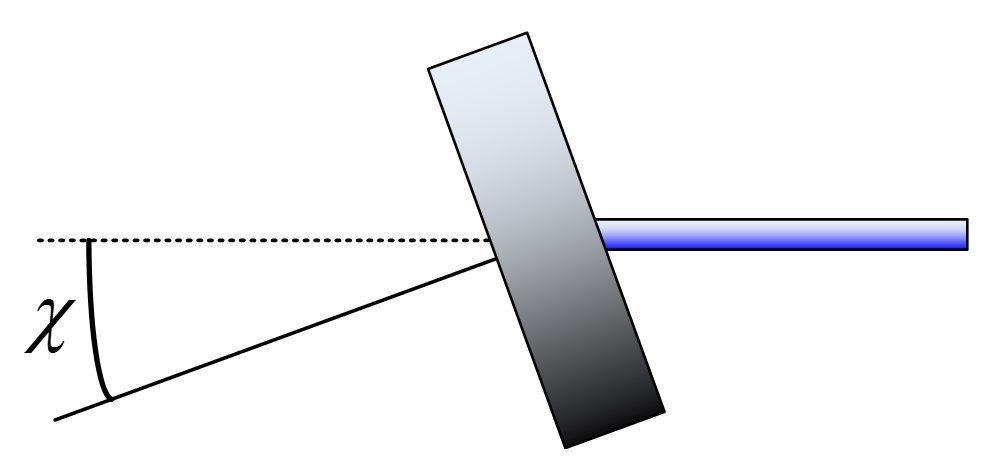
\includegraphics[width=.5\linewidth]{./figures/Images/Figure_1b}
	\caption{Depiction of skew angle $\chi$}
	\label{fig:ChiAngleDepiction}
	\centering
\end{figure}
\par
 Disk unbalance is caused by an eccentricity, or a geometrical distance between the axis of rotation and the center of mass of the disk. Eccentricity is represented here as $\epsilon$ and is equivalent to that geometric distance. The moment unbalance forces, the third and fourth equations of $ \vec{\mathbf{F}}^d $ in \eqref{eq:DiskNodeEquations}, are caused by the skew angle, $ \chi $, which is the angle the disk major axis forms with the axis of rotation as in Figure \ref{fig:ChiAngleDepiction}. The major axis is the axis normal from the disk face from which the polar moment of inertia, $ J_x $ is defined.
 \subsection{Disk in complex coordinates} \label{Disk in complex coordinates}
 Disk equations of motion \eqref{eq:DiskNodeEquationofMotion} are converted to the complex plane in the same manner the beam element was derived in \S\ref{Beam Element in Complex Coordinates}
 \begin{equation}\label{eq:DiskNodeEquationofMotionComplex}
 \bunderline{\mathbf{M}}^{dc}\ddot{\vec{\mathbf{q}}}^c_k-i\Omega\bunderline{\mathbf{G}}^{dc}\dot{\vec{\mathbf{q}}}^c_k=\Omega^2\vec{\mathbf{F}}^{dc}
 \end{equation}
 where,
 \begin{equation*}
 \bunderline{\mathbf{M}}^{dc}=\left[\begin{array}{cc}
 \rho Al&0\\
 0&\rho I
 \end{array}\right],\quad
 \bunderline{\mathbf{G}}^{dc}=\left[\begin{array}{cc}
 0&0\\
 0&\rho J_x
 \end{array}\right],\quad
 \vec{\mathbf{F}}^{dc}=\left\{\begin{array}{c}
 \rho A l \epsilon e^{i\delta_\epsilon}e^{i\Omega t}\\
 \rho(I-J_x)\chi e^{i\Omega t}
 \end{array}\right\}
 \end{equation*}
%\lstinputlisting[language=Matlab]{code/DiskMass.m}
%\lstinputlisting[language=Matlab]{code/DiskGyro.m}
\section{Bearing Nodal Equations} \label{Bearing Nodal Equations}
Bearings in this work are to be considered massless points of stiffness and damping acting at a node. Represented by the local equations of motion
\begin{equation}\label{eq:BearingNodeEquationsofMotion}
\bunderline{\mathbf{D}}^b\dot{\vec{\mathbf{q}}}_k+\bunderline{\mathbf{K}}^b\vec{\mathbf{q}}_k=0
\end{equation}
The superscript $ ^b $ indicates the matrix is for a bearing. A simple model for the stiffness and damping is used. Structural damping of the bearing is considered to be proportional to the stiffness, Raleigh Damping for the local bearing system. The stiffness matrix is comprised of only transverse stiffness terms, as 
\begin{equation}
\def\cs{2em}
\begin{array}{cc}
\bunderline{\mathbf{K}}^b=\left[\def\arraystretch{.8}\arraycolsep=0pt\begin{array}{cccccc}
\makebox[\cs]{$k_{yy}$}&\makebox[\cs]{$k_{yz}$}&\makebox[\cs]{0}&\makebox[\cs]{0}&\makebox[\cs]{0}&\makebox[\cs]{0}\\
k_{zy}&k_{zz}&0&0&0&0\\
0&0&0&0&0&0\\
0&0&0&0&0&0\\
0&0&0&0&0&0\\
0&0&0&0&0&0
\end{array}\right] & \bunderline{\mathbf{D}}^b=a\bunderline{\mathbf{K}}^b
\end{array}
\end{equation}
The stiffness is typically simplified further to represent an orthotropic bearing, where $ k_{yz}=k_{zy}=0 $ or further yet as a isotropic bearing, where $ k_{yz}=k_{zy}=0 $ \& $ k_{yy}=k_{zz}=k $. Generally, these unknown parameters of stiffness are determined by changing the values to achieve the correct natural frequencies of the system.
\subsection{Bearing in Complex Coordinates}
Following the same methodology as sections \S\ref{Beam Element in Complex Coordinates} \& \S\ref{Disk in complex coordinates}, the equation of motion in the complex plane is
\begin{equation}\label{eq:BearingNodeEquationsofMotionComplex}
\bunderline{\mathbf{D}}^{bc}\dot{\vec{\mathbf{q}}}^c_k+\bunderline{\mathbf{K}}^{bc}\vec{\mathbf{q}}^c_k=0
\end{equation}
where,
\begin{equation*}
 \bunderline{\mathbf{K}}^{bc}=\left[\begin{array}{cc}
k&0\\
0&k
\end{array}\right],\quad
\bunderline{\mathbf{D}}^{bc}=a\bunderline{\mathbf{K}}^{bc}
\end{equation*}
$ k $ is the isotropic bearing stiffness. It is possible to define the complex system with anisotropic terms of stiffness, but the complexity added to the system outweighs the benefit of using the complex plane in the first place.
%\lstinputlisting[language=Matlab]{code/BearingStiff.m}
%\lstinputlisting[language=Matlab]{code/BearingDamp.m}
\section{Assembly of the Global Systems of Equations} \label{Assembly of the Global Systems of Equations}
The matrices in the global system of equations are determined using the direct approach of taking the summation of the inertia, damping, stiffness, or force at each degree of freedom.
\subsection{In the Real Coordinate System}
\begin{equation}\label{eq:GlobalSystemofEquationsReal}
\bunderline{\mathbf{M}}\ddot{\vec{\mathbf{q}}}+\bunderline{\mathbf{G}}\dot{\vec{\mathbf{q}}}+\bunderline{\mathbf{K}}\vec{\mathbf{q}}=\Omega^2\vec{\mathbf{F}}
\end{equation}
Each summation is defined as 
\begin{equation*}
\left\{\begin{array}{rlrl}
\bunderline{\mathbf{M}}&=\bunderline{\mathbf{M}}^e_G+\bunderline{\mathbf{M}}^b_G+\bunderline{\mathbf{M}}^d_G&\bunderline{\mathbf{D}}&=\eta_v\bunderline{\mathbf{K}}^e_G+\Omega\bunderline{\mathbf{G}}^e_G+\Omega\bunderline{\mathbf{G}}^d_G+\bunderline{\mathbf{D}}^b_G\\
\bunderline{\mathbf{K}}&=\eta_a\bunderline{\mathbf{K}}^e_G+(\Omega\eta_v+\eta_b)\bunderline{\mathbf{C}}^e_G+\bunderline{\mathbf{K}}^b_G&\vec{\mathbf{F}}&=\vec{\mathbf{F}}^d_G
\end{array}\right.
\end{equation*}
Subscript $ _G $ indicates the matrix is in the global coordinate system that contains all of the degrees of freedom. Care must be taken here to associate the correct degrees of freedom, and recognize that some of the matrices are elemental and others are nodal. 
\subsection{In the Complex Coordinate System}
\begin{equation}\label{eq:GlobalSystemofEquationsComplex}
\bunderline{\mathbf{M}}\ddot{\vec{\mathbf{q}}}^c+\bunderline{\mathbf{D}}\dot{\vec{\mathbf{q}}}^c+\bunderline{\mathbf{K}}\vec{\mathbf{q}}^c=\Omega^2\vec{\mathbf{F}}
\end{equation}
where,
\begin{equation*}
\left\{\begin{array}{rlrl}
\bunderline{\mathbf{M}}&=\bunderline{\mathbf{M}}^{ec}_G+\bunderline{\mathbf{M}}^{dc}_G+\bunderline{\mathbf{M}}^{bc}_G&\bunderline{\mathbf{D}}&=\eta_v\bunderline{\mathbf{K}}^{ec}_G-i\Omega(\bunderline{\mathbf{G}}^{ec}_G+\bunderline{\mathbf{G}}^{dc}_G)+\bunderline{\mathbf{D}}^{bc}_G\\
\bunderline{\mathbf{K}}&=\eta_a\bunderline{\mathbf{K}}^{ec}_G-i(\Omega\eta_v+\eta_b)\bunderline{\mathbf{C}}^{ec}_G+\bunderline{\mathbf{K}}^{bc}_G&\vec{\mathbf{F}}&=\vect{F}^{dc}_G
\end{array}\right.
\end{equation*}
\section{Analysis of the Resulting Model}
A benefit of the finite element method is the resulting general linear Ordinary Differential Equations (ODEs) that are left to solve in equations \eqref{eq:GlobalSystemofEquationsReal} \& \eqref{eq:GlobalSystemofEquationsComplex}. Many techniques exist to provide frequency and time domain information on the solution of this system of equations. In their current state, equations \eqref{eq:GlobalSystemofEquationsReal} \& \eqref{eq:GlobalSystemofEquationsComplex} may be analyzed using frequency domain analysis techniques to be discussed in \S\ref{FrequencyDomainAnalysis}. On the other hand, in order to provide time domain solutions, numerical integration of these ODEs must be conducted. Details of the process of numerical integration is out of the scope of this work. Resulting time domain solutions of the ODEs for a specific nodal location can then be processed using the techniques outlined in \S\ref{VibrationSignalAnalysis}. This time domain method of processing the FEM model is vital in analyzing non-linear differential equations that may result from a more detailed model of bearings, asymmetry, and many other effects.\par